\documentclass[10pt,a4paper]{article}
\usepackage[utf8]{inputenc}
\usepackage[T1]{fontenc}
\usepackage[brazilian]{babel}
\usepackage[margin=1.7cm]{geometry}
\usepackage{booktabs}
\usepackage{enumitem}
\usepackage{xcolor}
\usepackage{graphicx}
\usepackage{tikz}
\usetikzlibrary{positioning,arrows.meta,shapes.multipart}
\usepackage[hidelinks]{hyperref}

\setlength{\parskip}{0.4em}
\setlength{\parindent}{0pt}
\setlist[itemize]{noitemsep, topsep=2pt, leftmargin=1.4em}
\setlist[enumerate]{itemsep=2pt, topsep=2pt, leftmargin=1.5em}
\sloppy

\definecolor{umlheader}{RGB}{230, 238, 248}
\definecolor{umlborder}{RGB}{60, 90, 130}
\definecolor{boxbg}{RGB}{246, 248, 252}

\begin{document}

% Cabeçalho Objetivo
\begin{center}
    {\Large \textbf{Relatório Técnico — Pong com Raylib-cs e Threads (POO)}}\\[0.25em]
    {\small Universidade Federal de São Paulo (Unifesp) — Programação Orientada a Objetos}\\[0.4em]
    {\small
    \begin{tabular}{ll@{\hspace{2.2cm}}ll}
        \textbf{Breno Porto Pinheiro do Prado} & RA: 185196 &
        \textbf{Felipe Pereira Silva} & RA: 188204 \\
        \textbf{Guilherme Bento Ramos} & RA: 185226 & & \\
    \end{tabular}}
\end{center}
\vspace{-0.2em}
\hrule
\vspace{0.4em}

\section*{1. Introdução e Objetivo}
Este trabalho apresenta o desenvolvimento de uma aplicação desktop do clássico jogo \textbf{Pong} (com temática de tênis de mesa) em \textbf{C\# (.NET 10)} utilizando a biblioteca gráfica \textbf{Raylib-cs} e \textbf{programação concorrente com Threads}. O objetivo principal é consolidar na prática os fundamentos de \textbf{Programação Orientada a Objetos (POO)} — como encapsulamento, construtores, associação/composição e separação de responsabilidades — aliados ao processamento concorrente seguro, separando o cálculo contínuo da física do jogo do fluxo principal de renderização da interface gráfica.

\section*{2. Funcionamento e Regras do Jogo}
A aplicação executa em janela HD ($1280 \times 720$ a 60 FPS, com MSAA 4x e VSync), exibindo uma mesa de tênis de mesa centralizada com espaçamento lateral externo para movimentação das duas raquetes, placar em tempo real e três botões interativos no topo:

\begin{itemize}
    \item \textbf{Controles de Partida:} \textbf{Iniciar Jogo} (inicia ou retoma a partida, também via tecla \texttt{ESPAÇO}), \textbf{Pausar Jogo} (suspende temporariamente a movimentação sem perder o placar, também via \texttt{ESPAÇO}) e \textbf{Reiniciar Jogo} (zera as pontuações e reposiciona bola e raquetes no centro, também via tecla \texttt{R}).
    \item \textbf{Movimentação das Raquetes:} O \textbf{Jogador 1} (raquete esquerda) utiliza as teclas \texttt{W} e \texttt{S}; o \textbf{Jogador 2} (raquete direita) utiliza as teclas \texttt{Seta para Cima} ($\uparrow$) e \texttt{Seta para Baixo} ($\downarrow$). Ambas têm suas coordenadas verticais restringidas (\textit{clamp}) aos limites superior e inferior da mesa.
    \item \textbf{Movimentação Contínua e Colisões da Bola:} A bola se desloca continuamente de forma autônoma. Ao colidir com as bordas superior ou inferior da mesa, inverte sua componente vertical (\texttt{ReverseY()}) e é reposicionada dentro do limite para evitar travamentos. Ao colidir com uma raquete, inverte a direção horizontal (\texttt{ReverseX(hitFactor)}), reposiciona-se na face externa da raquete (prevenindo atravessamento/\textit{tunelamento}), ajusta o ângulo de rebote conforme o ponto de impacto e recebe um ganho sutil de \textbf{+5\%} de velocidade por rebatida (de 440 px/s até o teto de 820 px/s) para tornar ralis longos progressivamente mais disputados.
    \item \textbf{Pontuação e Condição de Vitória:} Quando a bola ultrapassa a zona da raquete de um jogador, o adversário recebe \textbf{1 ponto} e a bola retorna ao centro da mesa na velocidade base, com nova direção inicial. A partida continua até que um dos jogadores alcance \textbf{5 pontos} (\texttt{WinningScore = 5}), momento em que o estado muda para \texttt{GameOver} e o vencedor é anunciado no painel central.
\end{itemize}

\newpage
\section*{3. Arquitetura da Aplicação e Diagrama de Classes UML}
O projeto adota uma arquitetura enxuta dividida em três módulos dentro de \texttt{src/} (\texttt{Models/}, \texttt{UI/} e \texttt{Game/}), além do ponto de entrada \texttt{Program.cs}, mapeando diretamente as entidades propostas na especificação (Bola, Raquete, Jogador, Jogo e Janela Principal) acrescidas do componente reutilizável \texttt{Button}.

\begin{center}
\begin{tikzpicture}[
    scale=0.84, transform shape,
    umlclass/.style={
        draw=umlborder,
        thick,
        rectangle split,
        rectangle split parts=3,
        rectangle split part fill={umlheader,white,white},
        font=\scriptsize\ttfamily,
        align=left,
        inner sep=3.5pt
    },
    umlenum/.style={
        draw=umlborder,
        thick,
        rectangle split,
        rectangle split parts=2,
        rectangle split part fill={umlheader,white},
        font=\scriptsize\ttfamily,
        align=left,
        inner sep=3.5pt
    },
    comp/.style={{Diamond[length=7pt,width=5pt]}-, thick, draw=umlborder},
    dep/.style={-{Stealth[length=5pt]}, dashed, thick, draw=umlborder}
]

% Program (Topo Esquerda)
\node[umlclass] (program) at (-6.8, 0.8) {
    \textbf{Program}
    \nodepart{second}
    + ScreenWidth : int = 1280\\
    + ScreenHeight : int = 720
    \nodepart{third}
    + Main() : void\\
    - ResolveAssetPath(string)
};

% PongGame (Centro Topo)
\node[umlclass] (game) at (0, 0) {
    \textbf{PongGame : IDisposable}
    \nodepart{second}
    - \_ball : Ball\\
    - \_player1, \_player2 : Player\\
    - \_btnStart, \_btnPause, \_btnRestart : Button\\
    - \_state : GameState\\
    - \_gameThread : Thread\\
    - \_pauseEvent : ManualResetEventSlim\\
    - \_cts : CancellationTokenSource\\
    - \_stateLock : object\\
    - \_uiActions : ConcurrentQueue<Action>
    \nodepart{third}
    + StartGame() : void\\
    + PauseGame() : void\\
    + RestartGame() : void\\
    + UpdateUI() : void\\
    + Draw(int, int) : void\\
    - GameLoopThread() : void\\
    - UpdatePhysicsLocked(float) : void\\
    - InvokeOnUiThread(Action) : void\\
    + Dispose() : void
};

% Button (Topo Direita)
\node[umlclass] (button) at (6.9, 1.1) {
    \textbf{Button}
    \nodepart{second}
    + Bounds : Rectangle\\
    + Text : string\\
    + IsEnabled : bool\\
    + BaseColor : Color
    \nodepart{third}
    + IsHovered() : bool\\
    + IsClicked() : bool\\
    + Draw(Font) : void
};

% GameState (Meio Direita)
\node[umlenum] (state) at (6.9, -2.0) {
    \textbf{<<enum>> GameState}
    \nodepart{second}
    NotStarted, Running,\\
    Paused, GameOver
};

% Ball (Abaixo Esquerda)
\node[umlclass] (ball) at (-6.5, -5.6) {
    \textbf{Ball}
    \nodepart{second}
    - \_position : Vector2\\
    - \_velocity : Vector2\\
    + Radius : float\\
    + BaseSpeed : float\\
    + MaxSpeed : float
    \nodepart{third}
    + Update(float) : void\\
    + ReverseX(float) : void\\
    + ReverseY() : void\\
    + SetPositionX/Y(float)\\
    + Reset(Vector2, int) : void
};

% Player (Abaixo Centro)
\node[umlclass] (player) at (0, -5.8) {
    \textbf{Player}
    \nodepart{second}
    + Name : string\\
    + Score : int\\
    + Paddle : Paddle\\
    + UpKey : KeyboardKey\\
    + DownKey : KeyboardKey
    \nodepart{third}
    + UpdateInput(float, float, float)\\
    + AddPoint() : void\\
    + ResetScore() : void
};

% Paddle (Abaixo Direita)
\node[umlclass] (paddle) at (6.7, -5.8) {
    \textbf{Paddle}
    \nodepart{second}
    - \_position : Vector2\\
    + Width : float\\
    + Height : float\\
    + Speed : float
    \nodepart{third}
    + MoveUp(float, float) : void\\
    + MoveDown(float, float) : void\\
    + Reset(float) : void\\
    + GetBounds() : Rectangle
};

% Relações
\draw[dep] (program.east) -- node[above, font=\scriptsize]{instancia} (game.west |- program.east);
\draw[comp] (game.east |- button.west) -- node[above, font=\scriptsize]{3} (button.west);
\draw[dep] (game.east |- state.west) -- node[above, font=\scriptsize]{estado} (state.west);
\draw[comp] (game.south west) -- node[left, font=\scriptsize]{1} (ball.north east);
\draw[comp] (game.south) -- node[left, font=\scriptsize]{2} (player.north);
\draw[comp] (player.east) -- node[above, font=\scriptsize]{1} (paddle.west);

\end{tikzpicture}
\end{center}

\section*{4. Classes Implementadas e Conceitos de POO Aplicados}
\begin{enumerate}
    \item \textbf{\texttt{Ball} (\texttt{src/Models/Ball.cs}):} Aplica \textbf{encapsulamento} mantendo os vetores \texttt{\_position} e \texttt{\_velocity} privados, expostos somente para leitura via propriedades e modificados apenas por métodos de domínio (\texttt{Update}, \texttt{ReverseX}, \texttt{ReverseY}, \texttt{SetPositionX/Y} e \texttt{Reset}). Seu \textbf{construtor} inicializa raio, posição e velocidades base/máxima.
    \item \textbf{\texttt{Paddle} (\texttt{src/Models/Paddle.cs}):} Encapsula posição (\texttt{\_position}), dimensões e velocidade da raquete. Garante a invariante de limites da mesa internamente nos métodos \texttt{MoveUp(dt, minY)} e \texttt{MoveDown(dt, maxY)}, fornecendo seu retângulo de colisão via \texttt{GetBounds()}.
    \item \textbf{\texttt{Player} (\texttt{src/Models/Player.cs}):} Representa cada jogador, encapsulando \texttt{Score} com escrita restrita (\texttt{private set}), alterável somente por \texttt{AddPoint()} e \texttt{ResetScore()}. Demonstra \textbf{composição/associação} ao agregar sua instância de \texttt{Paddle} e suas teclas de controle (\texttt{UpKey} e \texttt{DownKey}).
    \item \textbf{\texttt{Button} (\texttt{src/UI/Button.cs}):} Isola a responsabilidade de interface de botão clicável (geometria \texttt{Bounds}, texto, estado \texttt{IsEnabled}, cor, detecção de \textit{hover}/\textit{clique} e desenho arredondado com fonte vetorial).
    \item \textbf{\texttt{PongGame} (\texttt{src/Game/PongGame.cs}):} Classe orquestradora que demonstra \textbf{composição} de \texttt{Ball}, dois \texttt{Player}s e três \texttt{Button}s, implementando \texttt{IDisposable} para liberar os recursos de sincronização e encerrar a thread secundária. Mantém separação estrita entre lógica/física (\texttt{UpdatePhysicsLocked}), interação de UI (\texttt{UpdateUI}) e renderização (\texttt{Draw}).
    \item \textbf{\texttt{Program} (\texttt{Program.cs}):} Equivalente ao \texttt{FormulárioPrincipal} no ecossistema Raylib-cs; inicializa a janela gráfica, carrega a fonte vetorial suavizada (\texttt{font.otf}) e as texturas pixel-art (\texttt{table\_tennis.png}, \texttt{racket.png}, \texttt{ball.png}), executa o loop gráfico na thread principal e garante a chamada automática de \texttt{game.Dispose()} via bloco \texttt{using}.
\end{enumerate}

\section*{5. Programação Concorrente com Threads e Sincronização}
Para atender aos requisitos de concorrência sem congelar a interface e respeitando a restrição de afinidade de thread do contexto gráfico OpenGL (Raylib-cs), a aplicação divide a execução entre a \textbf{Thread Principal (UI/Renderização a 60 FPS)} e uma \textbf{Thread Dedicada de Processamento (\texttt{\_gameThread} a $\approx$120 Hz)}:

\begin{itemize}
    \item \textbf{Criação e Processamento Contínuo:} No construtor de \texttt{PongGame}, cria-se e inicia-se uma instância da classe \texttt{Thread} (de \texttt{System.Threading}, com \texttt{Name = "PongPhysicsThread"} e \texttt{IsBackground = true}) executando \texttt{GameLoopThread()}. Ela calcula o \textit{deltaTime} via \texttt{Stopwatch} e executa continuamente a leitura de movimentação, física da bola, colisões e verificação de pontos, independentemente de eventos de clique.
    \item \textbf{Pausa e Retomada sem \textit{Busy-Wait} (\texttt{ManualResetEventSlim}):} A primitiva \texttt{\_pauseEvent} inicia não sinalizada (\texttt{false}). Enquanto o jogo não estiver em \texttt{GameState.Running}, a thread permanece bloqueada em \texttt{\_pauseEvent.Wait(\_cts.Token)} com consumo nulo de CPU. Acionar \textbf{Iniciar/Retomar} ou \textbf{Reiniciar} executa \texttt{\_pauseEvent.Set()}, retomando imediatamente a física; acionar \textbf{Pausar} ou atingir 5 pontos executa \texttt{\_pauseEvent.Reset()}.
    \item \textbf{Exclusão Mútua (\texttt{lock}):} Todas as mutações de estado (posições, placar e \texttt{\_state}) e a leitura de \textit{snapshot} pela thread gráfica em \texttt{Draw()} são protegidas pelo monitor \texttt{lock (\_stateLock)}, eliminando condições de corrida (\textit{race conditions}) e leituras inconsistentes entre quadros.
    \item \textbf{Comunicação com a Thread de Interface (\texttt{ConcurrentQueue<Action>}):} Como o Raylib-cs utiliza um \textit{game loop} explícito em vez do loop de mensagens do Windows Forms (\texttt{Invoke}/\texttt{BeginInvoke}), implementou-se o padrão equivalente através do método \texttt{InvokeOnUiThread(Action)}, que enfileira atualizações de interface (como a mensagem de vitória e o estado dos botões ao encerrar a partida) na fila concorrente \texttt{\_uiActions}, drenada e executada de forma segura pela thread principal no início de cada quadro em \texttt{UpdateUI()}.
    \item \textbf{Encerramento Seguro (\texttt{CancellationTokenSource} + \texttt{Join}):} Ao fechar a janela, o bloco \texttt{using} em \texttt{Program.cs} invoca \texttt{PongGame.Dispose()}, que aciona \texttt{\_cts.Cancel()}, desbloqueia a thread caso esteja pausada (\texttt{\_pauseEvent.Set()}) e aguarda seu término limpo via \texttt{\_gameThread.Join()}, impedindo threads órfãs após o fechamento da aplicação.
\end{itemize}

\section*{6. Capturas de Tela da Aplicação}
\begin{center}
    \setlength{\fboxsep}{0pt}
    \begin{minipage}[t]{0.48\textwidth}
        \centering
        \fbox{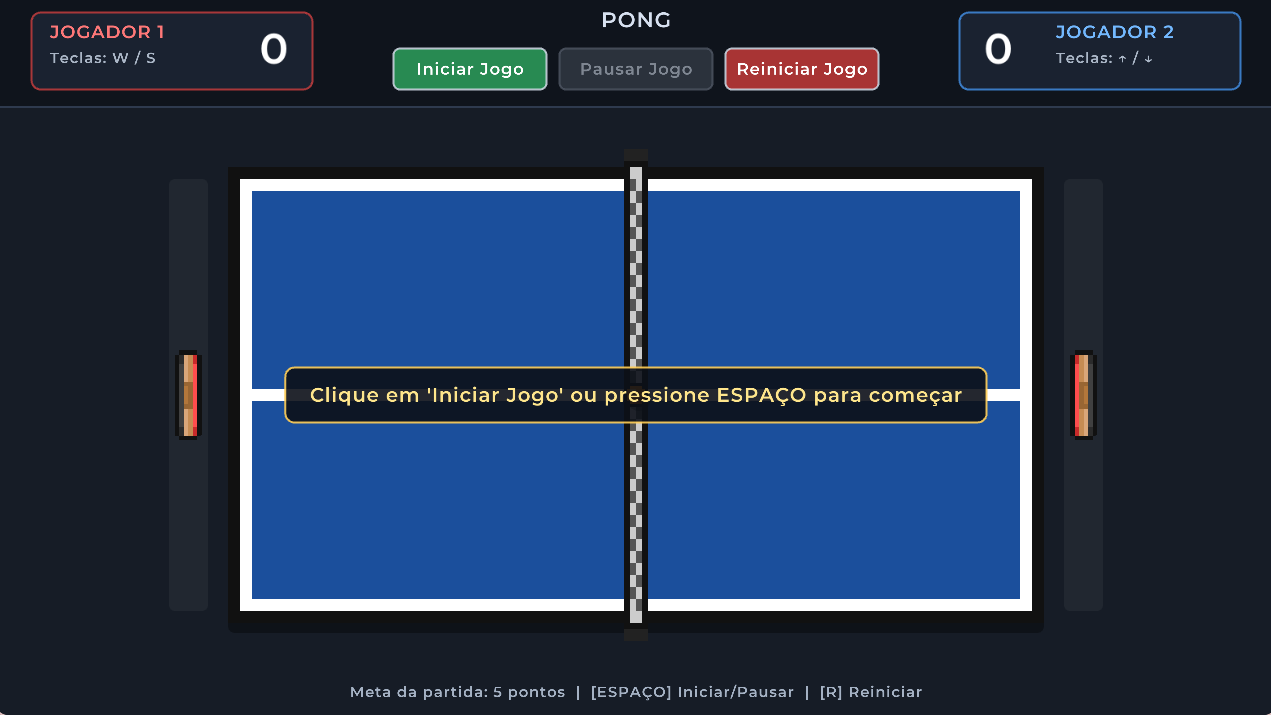
\includegraphics[width=\dimexpr\textwidth-2\fboxrule\relax]{prints/tela_inicial.png}}\\[0.3em]
        {\footnotesize\textbf{Figura 1:} Tela inicial (\texttt{NotStarted}) com mesa centralizada, raquetes nas laterais externas e controles no topo.}
    \end{minipage}\hfill
    \begin{minipage}[t]{0.48\textwidth}
        \centering
        \fbox{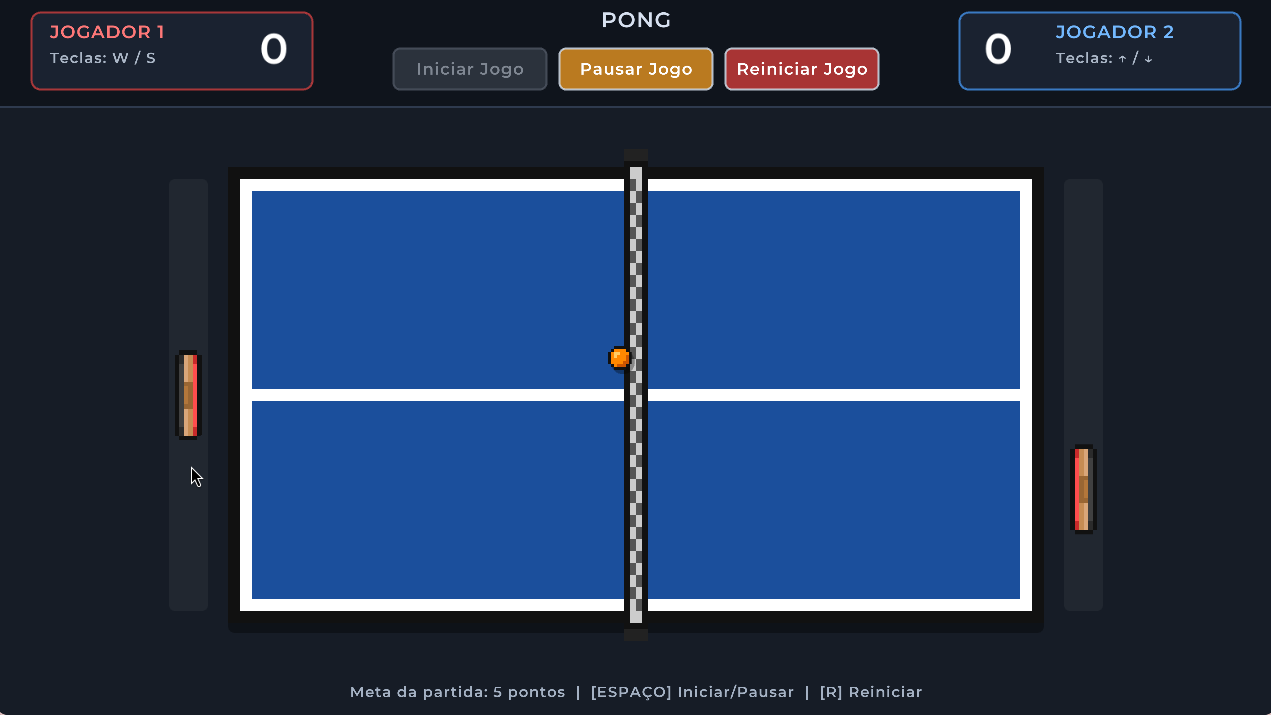
\includegraphics[width=\dimexpr\textwidth-2\fboxrule\relax]{prints/partida_em_andamento.png}}\\[0.3em]
        {\footnotesize\textbf{Figura 2:} Partida em andamento (\texttt{Running}) com a bola em movimento contínuo pela thread de física.}
    \end{minipage}

    \vspace{0.7em}

    \begin{minipage}[t]{0.52\textwidth}
        \centering
        \fbox{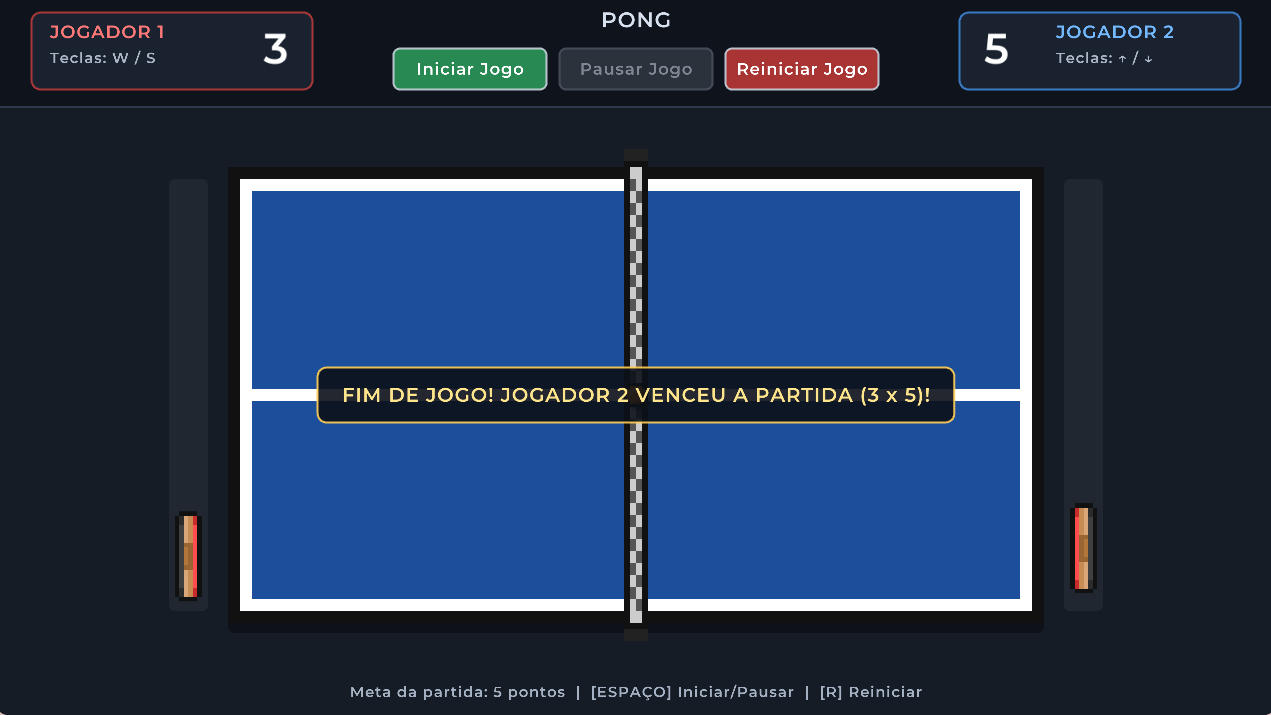
\includegraphics[width=\dimexpr\textwidth-2\fboxrule\relax]{prints/fim_de_jogo.png}}\\[0.3em]
        {\footnotesize\textbf{Figura 3:} Encerramento da partida (\texttt{GameOver}) ao atingir a meta de 5 pontos com anúncio do vencedor.}
    \end{minipage}
\end{center}

\section*{7. Repositório do Projeto}
\begin{itemize}
    \item \textbf{Repositório GitHub:} \url{https://github.com/brenoprato/projetos-POO} (diretório \texttt{pong/})
\end{itemize}

\end{document}
